%\setchapterimage{Fond_SLCI.png}
\setchapterpreamble[u]{\margintoc}
\chapter{Algorithmes gloutons}

%\marginnote[5cm]{
%\UPSTIcompetence[2]{C1-02}
%\UPSTIcompetence[2]{C2-04}
%}

%\marginnote[4cm]{\textbf{Qui}, \textit{Quoi}, Où.}


\section{Présentation des algorithmes Gloutons}

\textit{
En informatique, un algorithme glouton (greedy algorithm en anglais, parfois appelé aussi algorithme gourmand) est un algorithme qui suit le principe de faire, étape par étape, un choix optimum local. Dans certains cas, cette approche permet d'arriver à un optimum global, mais dans le cas général c'est une heuristique \sidenote{Une heuristique est une méthode de calcul qui fournit rapidement une solution réalisable, pas nécessairement optimale ou exacte, pour un problème d'optimisation difficile.}} (Wikipédia).\\

Les algorithmes gloutons sont utilisés dans des problèmes d’optimisation. Un problème d’optimisation consiste à déterminer les valeurs des paramètres permettant de :
\begin{itemize}
	\item minimiser ou maximiser une fonction objectif ;
	\item satisfaire une ou des fonctions contraintes (il existe des problèmes avec ou sans contrainte).
\end{itemize}

\subsection{Choix d'itinéraire}
 
On peut citer par exemple le problème du choix d’itinéraire dans un réseau routier : il faut déterminer le trajet de sorte à minimiser le temps de parcours, tout en respectant un ensemble de contraintes : circuler sur les routes (on ne coupe pas à travers champs !) et respecter les sens de circulation.

\subsection{Recherche d'un minimum d'une fonction} 

\begin{itemize}
	\item 	La recherche du minimum de la fonction $f:x \longmapsto x^2-x-2$ est un problème d’optimisation sans contrainte.
	\item		La recherche du minimum de la fonction $f:x \longmapsto x^2-x-2$ sous la contrainte $x^3\geq8$ est un problème d’optimisation sous contrainte (contrainte d’inégalité). L’optimum est alors $x=2$ et $f(2)=0$. L’ensemble des solutions vérifiant les contraintes sont appelées solutions valides ou valables.
\end{itemize}



\begin{marginfigure}
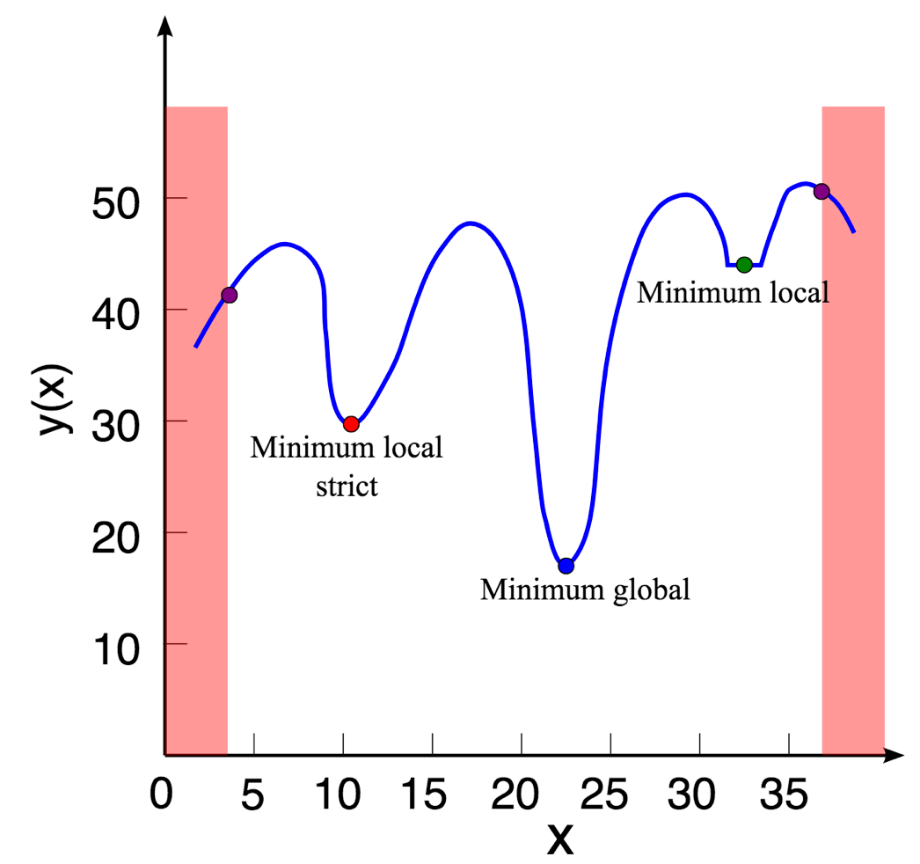
\includegraphics[width=\linewidth]{optimums.png}
\end{marginfigure}


On distingue également plusieurs types d’optimum :
\begin{itemize}
	\item optimum global ;
	\item	optimum local strict (unique dans un intervalle réduit);
	\item	optimum local (non unique dans un intervalle réduit).
\end{itemize}

La méthode gloutonne est très puissante et fonctionne bien pour toutes sortes de problèmes. L'algorithme de \lstinline{Dijkstra}, que l'on étudiera en fin d'année, qui calcule des plus courts chemins à origine unique, peut être vu comme une application de la méthode gloutonne.

\subsection{\'Eléments de la stratégie gloutonne}

Le processus pour mettre au point un algorithme glouton présente plusieurs étapes :

\begin{enumerate}
\item Détermination de la sous-structure optimale du problème ;
\item Développement d'une solution formulée par récurrence ;
\item Démonstration que, si nous avons fait un choix glouton, il ne reste qu'un seul sous-problème ;
\item Démonstration qu'il est toujours sûr de faire le choix glouton. (Les étapes 3 et 4 peuvent se faire dans n'importe quel ordre.)
\item \'Ecriture d'un algorithme récursif ou itératif.
\end{enumerate}

\subsection{Propriété de choix glouton}

La première caractéristique principale est la propriété de choix glouton : on peut assembler une solution globalement optimale en effectuant des choix localement optimaux (gloutons). Autrement dit, quand on considère le choix à faire, on fait le choix qui paraît le meilleur pour le problème courant, sans tenir compte des résultats des sous-problèmes.


\subsection{Exemple : un problème d'organisation \sidenote{Source : algorithmes gloutons - eduscol}}



Des conférenciers sont invités à présenter leurs exposés dans une salle. Mais leurs disponibilités ne leur permettent d'intervenir qu'à des horaires bien définis. Le problème est de construire un planning d'occupation de la salle avec le plus grand nombre de conférenciers.\\
Désignons par $n$, entier naturel non nul, le nombre de conférenciers. Chacun d'eux, identifié par une lettre $C_i$, où $i$ est un entier compris entre 0 et $n-1$, est associé à un intervalle temporel \verb![!di, fi\verb![! où di et fi désignent respectivement l'heure de début et l'heure de fin de l'intervention. Afin de dégager une tactique de résolution du problème, commençons par analyser plusieurs situations.

\paragraph*{Les créneaux ne se chevauchent pas}

Une telle situation est simple puisque tous les conférenciers peuvent intervenir sur des créneaux horaires disjoints.

\paragraph*{Les créneaux se chevauchent}

Dans cette situation, les intervalles ne sont plus disjoints. Nous dirons que ces intervalles ne sont pas compatibles. Des choix doivent être faits et certains conférenciers peuvent ne pas être retenus pour construire un planning.



%\newpage
%\renewcommand{\contentsname}{Plan du cours}
%\tableofcontents




